\documentclass[a4paper,11pt]{article}
\usepackage[utf8]{inputenc}
\usepackage{geometry}
\geometry{margin=1in}
\usepackage{graphicx}
\usepackage{listings}
\usepackage{xcolor}
\usepackage{hyperref}
\usepackage{booktabs}
\usepackage{longtable}
\usepackage{tikz}
\usetikzlibrary{shapes.geometric, arrows.meta, positioning}
\usepackage{amsmath}
\usepackage{amssymb}

% Code listing style
\definecolor{codegreen}{HTML}{28A745}
\definecolor{codegray}{HTML}{6C757D}
\definecolor{codeblue}{HTML}{2E86AB}
\definecolor{codepurple}{HTML}{9B59B6}
\definecolor{codeorange}{HTML}{FF9F43}
\definecolor{backcolour}{HTML}{F8F9FA}

\lstdefinestyle{mystyle}{
    backgroundcolor=\color{backcolour},
    commentstyle=\color{codegreen},
    keywordstyle=\color{codeblue},
    numberstyle=\tiny\color{codegray},
    stringstyle=\color{codeorange},
    basicstyle=\ttfamily\footnotesize,
    breakatwhitespace=false,
    breaklines=true,
    captionpos=b,
    keepspaces=true,
    numbers=left,
    numbersep=5pt,
    showspaces=false,
    showstringspaces=false,
    showtabs=false,
    tabsize=2,
    language=Python
}
\lstset{style=mystyle}

% Colors
\definecolor{jkcGold}{HTML}{F7931A}
\definecolor{jkcBlue}{HTML}{2E86AB}
\definecolor{jkcGreen}{HTML}{28A745}

\title{\textbf{UTXO-VM Technical Specification}\\
\large Junkcoin Cross-Chain Settlement Layer\\
\large Protocol \& Architecture Document}
\author{UTXO-VM Development Team}
\date{\today}

\begin{document}

\maketitle

\begin{abstract}
This document specifies the UTXO-VM protocol, a chain-agnostic smart object execution framework for UTXO-based blockchains. UTXO-VM enables Junkcoin (JKC) to function as a cross-chain settlement layer for AuxPow chains through a dual execution model: native opcodes for performance-critical operations and inscription envelopes for universal compatibility. The protocol achieves Turing-complete execution while maintaining the security properties of UTXO-based accounting through Single-Use Seals.
\end{abstract}

\tableofcontents

\newpage

\section{Executive Summary}

UTXO-VM is a clean-room, patent-free smart object execution framework that enables:

\begin{itemize}
    \item \textbf{Cross-chain settlement}: Junkcoin serves as the settlement layer for AuxPow UTXO chains
    \item \textbf{Dual execution model}: Native opcodes (primary) + inscription envelopes (fallback)
    \item \textbf{Universal compatibility}: Works on any Bitcoin-like chain without protocol changes
    \item \textbf{State management}: Single-Use Seals for deterministic state transitions
    \item \textbf{WASM execution}: Wasmtime-based runtime for smart contracts
\end{itemize}

\subsection{Key Metrics}
\begin{table}[h]
\centering
\begin{tabular}{@{}ll@{}}
\toprule
\textbf{Metric} & \textbf{Value} \\
\midrule
Testnet Transactions & 28+ \\
Smart Objects Indexed & 25+ \\
Test Pass Rate & 100\% (13/13) \\
Supported Chains & 13 \\
Opcodes Implemented & 5 \\
Block Height & 164,900+ \\
\bottomrule
\end{tabular}
\caption{Current Implementation Status}
\end{table}

\section{Architecture Overview}

\subsection{System Components}

\begin{figure}[h]
\centering
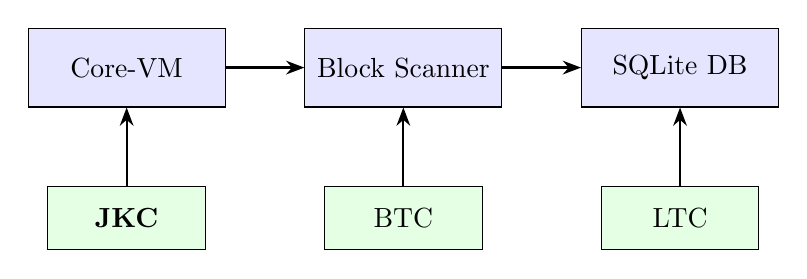
\begin{tikzpicture}[
  node distance=1cm,
  block/.style={rectangle, draw=black, fill=blue!10, minimum width=2.5cm, minimum height=1cm, align=center},
  chain/.style={rectangle, draw=black, fill=green!10, minimum width=2cm, minimum height=0.8cm, align=center},
  arrow/.style={-Stealth, thick},
]

% Core Components
\node[block] (vm) {Core-VM};
\node[block, right=of vm] (scanner) {Block Scanner};
\node[block, right=of scanner] (db) {SQLite DB};

% Chains
\node[chain, below=of vm] (jkc) {\textbf{JKC}};
\node[chain, below=of scanner] (btc) {BTC};
\node[chain, below=of db] (ltc) {LTC};

% Connections
\draw[arrow] (vm) -- (scanner);
\draw[arrow] (scanner) -- (db);
\draw[arrow] (jkc) -- (vm);
\draw[arrow] (btc) -- (scanner);
\draw[arrow] (ltc) -- (db);

\end{tikzpicture}
\caption{UTXO-VM System Architecture}
\end{figure}

\subsection{Data Flow}

\begin{enumerate}
    \item \textbf{Block Ingestion}: Scanner fetches blocks from electrs API
    \item \textbf{Transaction Parsing}: OP\_RETURN outputs analyzed for envelopes/opcodes
    \item \textbf{Execution}: Envelopes processed via inscription parser; opcodes via native handler
    \item \textbf{State Update}: Single-Use Seals spent and created for state transitions
    \item \textbf{Persistence}: State stored in SQLite with WAL mode
\end{enumerate}

\section{Protocol Specification}

\subsection{Wire Format: Inscription Envelope}

The UTXO-VM protocol uses Bitcoin's OP\_RETURN and witness script mechanisms to embed data:

\begin{lstlisting}[language={}, caption={Envelope Structure}]
OP_FALSE OP_IF
  OP_PUSH "utxovm"              # Protocol Identifier (6 bytes)
  OP_PUSH <version>             # Protocol Version (1 byte)
  OP_PUSH <contentType>         # MIME Type (variable)
  OP_PUSH <payload>             # Contract/Call Data (variable)
OP_ENDIF
\end{lstlisting}

\subsection{ScriptPubKey Encoding}

\begin{lstlisting}[language={}, caption={Example: Deploy Contract}]
# OP_RETURN + PushData + Envelope
6a                          # OP_RETURN
4c 2d                       # PUSHDATA1, 45 bytes
00                          # OP_FALSE
63                          # OP_IF
  06 7574786f766d            # PUSH "utxovm" (6 bytes)
  01 01                      # PUSH version 1
  10 6170706c69636174696f...  # PUSH "application/json" (16 bytes)
  0f 7b226e616d65223a22...   # PUSH payload (15 bytes)
68                          # OP_ENDIF
\end{lstlisting}

\subsection{Content Types}

\begin{table}[h]
\centering
\begin{tabular}{@{}ll@{}}
\toprule
\textbf{Content Type} & \textbf{Purpose} \\
\midrule
application/wasm & Deploy WASM smart contract \\
application/json & Execute method call \\
application/octet-stream & Raw data inscription \\
\bottomrule
\end{tabular}
\caption{Supported Content Types}
\end{table}

\section{Opcode Specification}

\subsection{JKC Native Opcodes}

When Junkcoin enables opcode support, the following opcodes are available:

\begin{table}[h]
\centering
\begin{tabular}{@{}clll@{}}
\toprule
\textbf{Opcode} & \textbf{Name} & \textbf{Input} & \textbf{Output} \\
\midrule
0xc0 & OP\_CREATE\_SMART\_OBJECT & JSON & Object ID \\
0xc1 & OP\_CALL\_SMART\_OBJECT & JSON & State Hash \\
0xc2 & OP\_UPDATE\_STATE & JSON & State Hash \\
0xc3 & OP\_SETTLE\_CROSS\_CHAIN & JSON & Settlement ID \\
0xc4 & OP\_VERIFY\_SEAL & JSON & Boolean \\
\bottomrule
\end{tabular}
\caption{JKC Opcode Table}
\end{table}

\subsection{Opcode Format}

\begin{lstlisting}[language={}, caption={Opcode Structure}]
# ScriptPubKey for OP_CREATE_SMART_OBJECT
c0                          # Opcode: CREATE_SMART_OBJECT
{                           # JSON Payload
  "codeHash": "0x...",
  "wasmHex": "0061736d...",
  "owner": "address",
  "satoshis": "1000",
  "initialState": {...}
}
\end{lstlisting}

\section{State Management}

\subsection{Single-Use Seals}

Every smart object is bound to a UTXO via a \textbf{Single-Use Seal}:

\begin{itemize}
    \item \textbf{Seal Format}: \texttt{txid:vout} (e.g., \texttt{abc123...:0})
    \item \textbf{State Transition}: Spending a seal creates a new seal
    \item \textbf{Deterministic}: Same input state + method = same output state
\end{itemize}

\subsection{State Transition Record}

\begin{lstlisting}[language=Python, caption={State Transition}]
{
  "objectId": "obj_abc123...",
  "txid": "def456...",
  "consumedSeal": "abc123...:0",
  "newSeal": "def456...:0",
  "method": "transfer",
  "events": [
    {
      "topic": "Transfer",
      "data": "1000 tokens transferred"
    }
  ],
  "blockHeight": 164900,
  "timestamp": 1693776000000
}
\end{lstlisting}

\section{Cross-Chain Settlement}

\subsection{Settlement Architecture}

\begin{figure}[h]
\centering
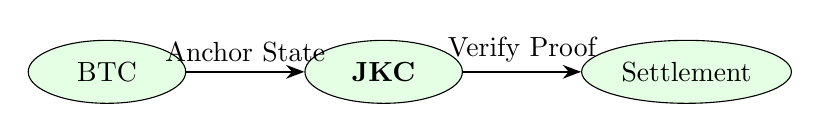
\begin{tikzpicture}[
  node distance=1.5cm,
  chain/.style={ellipse, draw=black, fill=green!10, minimum width=2cm, minimum height=0.8cm, align=center},
  arrow/.style={-Stealth, thick},
]

% Chains
\node[chain] (btc) {BTC};
\node[chain, right=of btc] (jkc) {\textbf{JKC}};
\node[chain, right=of jkc] (settlement) {Settlement};

% Connections
\draw[arrow] (btc) -- node[above] {Anchor State} (jkc);
\draw[arrow] (jkc) -- node[above] {Verify Proof} (settlement);

\end{tikzpicture}
\caption{Cross-Chain Settlement Flow}
\end{figure}

\subsection{Settlement Process}

\begin{enumerate}
    \item \textbf{Child Chain}: Creates state anchor with Merkle proof
    \item \textbf{Anchor Transaction}: Broadcast to JKC via OP\_SETTLE\_CROSS\_CHAIN
    \item \textbf{Verification}: JKC validates Merkle proof and state root
    \item \textbf{Settlement}: State recorded on JKC settlement layer
    \item \textbf{Claim}: Child chain can claim settled state
\end{enumerate}

\section{Core Components}

\subsection{Core-VM (Rust)}

The WASM execution engine built with Wasmtime:

\begin{lstlisting}[language=Python, caption={VM Execution}]
pub fn execute(
    wasm_bytes: &[u8],
    state: &[u8],
    caller: &str,
    method: &str,
    args: &[u8],
) -> Result<ExecutionResult, VMError> {
    // 1. Validate WASM module
    // 2. Instantiate with host functions
    // 3. Execute method with gas metering
    // 4. Return updated state
}
\end{lstlisting}

\subsection{Indexer (TypeScript)}

Block scanner with electrs integration:

\begin{lstlisting}[language=Python, caption={Scanner Logic}]
async processTransaction(tx: BlockTransaction) {
  // Check for opcodes first (JKC)
  const opcode = detectOpcode(tx.scriptPubKey);
  if (opcode) {
    return processOpcode(opcode, tx);
  }
  
  // Fallback to inscription parsing
  const envelope = parseEnvelope(tx.opReturn);
  if (envelope) {
    return processEnvelope(envelope, tx);
  }
}
\end{lstlisting}

\subsection{SQLite Database}

Persistent storage with WAL mode:

\begin{table}[h]
\centering
\begin{tabular}{@{}ll@{}}
\toprule
\textbf{Table} & \textbf{Purpose} \\
\midrule
objects & Smart object records \\
state\_transitions & State transition history \\
sync\_state & Chain sync status \\
\bottomrule
\end{tabular}
\caption{Database Schema}
\end{table}

\section{API Reference}

\subsection{Endpoints}

\begin{longtable}{@{}lll@{}}
\toprule
\textbf{Method} & \textbf{Endpoint} & \textbf{Description} \\
\midrule
\endhead
GET & /api/v1/chain/info & Chain information \\
GET & /api/v1/chains & Available chains \\
GET & /api/v1/objects & All smart objects \\
GET & /api/v1/object/:id & Get object by ID \\
GET & /api/v1/object/:id/history & State transitions \\
POST & /api/v1/sync & Sync from electrs \\
GET & /api/v1/sync/status & Sync status \\
POST & /api/v1/mempool/scan & Scan mempool \\
POST & /api/v1/parse-envelope & Parse envelope \\
POST & /api/v1/broadcast & Broadcast transaction \\
\bottomrule
\end{longtable}

\section{Deployment}

\subsection{Docker}

\begin{lstlisting}[language=Python, caption={Docker Compose}]
# Testnet
CHAIN=JKC_TESTNET docker-compose up -d

# Mainnet (when opcodes enabled)
docker-compose --profile mainnet up -d
\end{lstlisting}

\subsection{Environment Variables}

\begin{table}[h]
\centering
\begin{tabular}{@{}ll@{}}
\toprule
\textbf{Variable} & \textbf{Default} \\
\midrule
CHAIN & JKC\_TESTNET \\
CHAIN\_CONFIG\_PATH & ./chain.json \\
DB\_PATH & ./data/indexer.db \\
SYNC\_INTERVAL\_MS & 30000 \\
PORT & 9773 \\
\bottomrule
\end{tabular}
\caption{Environment Configuration}
\end{table}

\section{Security Considerations}

\begin{itemize}
    \item \textbf{Deterministic Execution}: Same input always produces same output
    \item \textbf{Gas Metering}: Prevents infinite loops and DoS attacks
    \item \textbf{Single-Use Seals}: Prevents double-spending of state
    \item \textbf{Merkle Proofs}: Verifiable cross-chain state anchoring
    \item \textbf{WASM Sandboxing}: Isolated execution environment
\end{itemize}

\section{Future Work}

\begin{enumerate}
    \item \textbf{Mainnet Opcodes}: Enable native opcodes on JKC mainnet
    \item \textbf{Child Chain Integration}: Connect BTC, LTC, DOGE settlement
    \item \textbf{Privacy Extensions}: MWEB integration for confidential transactions
    \item \textbf{Mempool Indexing}: Real-time unconfirmed transaction tracking
    \item \textbf{Production Monitoring}: Observability and alerting
\end{enumerate}

\appendix

\section{Test Results}

\begin{table}[h]
\centering
\begin{tabular}{@{}ll@{}}
\toprule
\textbf{Test Suite} & \textbf{Result} \\
\midrule
Token E2E & 6/6 PASS \\
Sequential Chain & 11/11 PASS \\
Comprehensive Suite & 13/13 PASS \\
Cross-Chain Anchor & 7/7 PASS \\
Persistence & 12/12 PASS \\
\midrule
\textbf{Total} & \textbf{49/49 PASS} \\
\bottomrule
\end{tabular}
\caption{Test Results Summary}
\end{table}

\section{Glossary}

\begin{description}
    \item[AuxPow] Auxiliary Proof of Work - merge mining mechanism
    \item[Single-Use Seal] Cryptographic primitive that can only be consumed once
    \item[Envelope] Data structure embedded in OP\_RETURN outputs
    \item[Opcode] Native instruction executed by the blockchain
    \item[Settlement] Process of anchoring state from child chain to settlement layer
    \item[WASM] WebAssembly - binary instruction format for stack-based virtual machines
\end{description}

\end{document}
